\selectlanguage{ngerman}
\begin{ledgroupsized}[r]{120mm}
\footnotesize
\pstart
\noindent\textbf{Überlieferung:}
\pend
\end{ledgroupsized}
\begin{ledgroupsized}[r]{114mm}
\footnotesize
\pstart \parindent -6mm
\makebox[6mm][l]{\textit{L}}%
Aufzeichnung:
LH~XXXVII~5 Bl.\;44.
Ein Blatt~2\textsuperscript{o},
unterer Rand ausgefranst mit geringfügigem Textverlust;
Papiererhaltungsmaßnahmen.
Ein \href{\Scan{LH_37_05_044wz}}{Wasserzeichen} mittig:
Papier der Klostermühle zu Thierhaupten bei Augsburg.%
\indexO{Thierhaupten bei Augsburg}\indexO{Augsburg}
Eine vollbeschriebene Seite auf Bl.\;44\,r\textsuperscript{o}
und vier Zeilen auf Bl.\;44\,v\textsuperscript{o},
sonst unbeschrieben.
Sämtliche Diagramme eigenhändig von Leibniz nummeriert.
\pend%
\end{ledgroupsized}%
\vspace{5mm}%
\begin{ledgroup}%
\footnotesize%
\pstart%
\noindent%
\textbf{Datierungsgründe:}%
\pagelabel{LH_37_05_044_datierung}
Die undatierte Aufzeichnung N.\;\ref{60300} \textit{De impulsu eccentrico} ist auf Papier der Klostermühle zu Thierhaupten bei Augsburg\indexO{Augsburg} verfasst.\indexO{Thierhaupten bei Augsburg}
Leibniz hielt sich in Augsburg\indexO{Augsburg} und Regensburg\indexO{Regensburg} im April 1690 auf, als er sich nach seiner Italienreise\indexO{Italien} auf dem Weg von Venedig\indexO{Venedig} nach Wien\indexO{Wien} befand (\textit{Chronik}, S.\;102\,f.).\cite{01236}
Die Aufzeichnung N.\;\ref{60300} wurde wohl damals geschrieben.
Die in \textit{LSB} VIII,\;3 N.\;31\textsubscript{2} edierte \textit{Appendix de vi absoluta},\cite{01397} deren Reinschrift \textit{L\textsuperscript{2}} auf gleichem Papier der Abtei zu Thierhaupten\indexO{Thierhaupten bei Augsburg} abgefasst wurde, zeigt, dass Leibniz seinen bairischen Aufenthalt unter anderem nutzte, um einige in den letzten Monaten seiner Italienreise\indexO{Italien} entstandene Entwürfe weiter zu bearbeiten.
Ähnlich dürfte es sich auch mit der Aufzeichnung N.\;\ref{60300} \textit{De impulsu eccentrico} verhalten.
Denn wie die auf \refpassage{LH_37_05_044r_alias_dhe-1}{LH_37_05_044r_alias_dhe-2} anzutreffende Anspielung zeigt, nimmt N.\;\ref{60300} unmittelbar auf die Behandlung des exzentrischen Stoßes in dem wohl noch Ende 1689 oder Anfang 1690 in Oberitalien\indexO{Italien} verfassten Text N.\;\ref{60142+60297} Bezug, um die dort (\refpassage{60142+60297_centrumgyrationis-1}{60142+60297_centrumgyrationis-2}) geäußerte Ansicht über das \textit{centrum gyrationis} zu berichtigen:
Anders als in N.\;\ref{60142+60297} ist Leibniz in N.\;\ref{60300} überzeugt, dass der Mittelpunkt der vom exzentrischen Stoß herrührenden Drehung mit dem Schwerpunkt des gesamten angestoßenen Körpers zusammenfalle.
Auch die Aufzeichnung N.\;\ref{60300} ist somit \textendash\ wie die Reinschrift \textit{LSB} VIII,\;3 N.\;31\textsubscript{2}, \textit{L\textsuperscript{2}} \textendash\ aller Wahrscheinlichkeit nach auf April 1690 zu datieren.
\pend%
\pstart%
Ferner gilt es zu beachten, dass kurz vor seiner Abreise aus Venedig\indexO{Venedig} Leibniz in seinem Brief an Rudolf Christian von Bodenhausen\indexN{\textls{Bodenhausen} (Bodenus, Bodenausen), Rudolf Christian, Freiherr v. 1698} vom 18.\;März 1690 versprochen hatte, den der Stoßlehre gewidmeten, noch unvollständigen Abschnitt der \textit{Dynamica} (%
\textit{CFP}~I, S.\;392--445~\bracks{A}; II.2, S.\;490--550~\bracks{C})\cite{01354} auf dem Weg nach Augsburg\indexO{Augsburg} abzuschließen (\textit{LSB} III,\;4 N.\;245, S.\;485.15\textendash23;\cite{01392} siehe zudem \textit{LSB} III,\;4 N.\;242, S.\;473.25\textendash474.1).\cite{01390}
Die Aufzeichnung N.\;\ref{60300} könnte somit ein vorläufiges Ergebnis aus Leibnizens Bestreben darstellen, die Versprechung an Bodenhausen\indexN{\textls{Bodenhausen} (Bodenus, Bodenausen), Rudolf Christian, Freiherr v. 1698} zu erfüllen.
(Siehe über die Genese der \textendash\ nie vollendeten \textendash\ \textit{Dynamica}\cite{01354} unter besonderer Berücksichtigung der Stoßlehre die einleitende Erläuterung zu N.\;\ref{impulsuseccentricus}, \refpassage{impulsecc_intro_Dynam-1}{impulsecc_intro_Dynam-2}.)
Auch dies bekräftigt die Annahme, dass die Aufzeichnung N.\;\ref{60300} im April 1690 entstand.
\pend%
\pstart%
Selbst wenn Leibniz erst später \textendash\ auf der Rückfahrt nach Hannover\indexO{Hannover} oder gar am Zielort \textendash\ die Aufzeichnung N.\;\ref{60300} verfasst haben sollte, so ist diese letztere in jedem Fall vor den von ihm eigenhändig auf den 31.\;Okto\-ber\,/\,10.\;November 1690 datierten \textit{Schedae de concursu eccentrico} N.\;\ref{58940} und N.\;\ref{58939} entstanden.
Denn über den Mittelpunkt der Drehung wird dort (N.\;\ref{58940}, \refpassage{LH_35_11_14_005-006_005r_cntrgyr-1}{LH_35_11_14_005-006_005r_cntrgyr-2}) ohne weitere Bemerkungen dieselbe Ansicht vertreten wie in der Aufzeichnung N.\;\ref{60300}.
\pend%
\end{ledgroup}%
\selectlanguage{latin}%
\frenchspacing%
\newpage%
\pstart%
\normalsize%
\noindent%
\lbrack%
\href{\Scan{LH_37_05_044r}}%
{44\,r\textsuperscript{o}}%
\rbrack\ %
\hfill%
De impulsu Eccentrico%
\indexS{impulsus eccentricus}%
\hfill%
\phantom{\lbrack44\,r\textsuperscript{o}\rbrack}%
\pend%
\vspace{1.0em}%
\pstart%
\noindent%
Cum recta \textit{AB}%
\indexS{recta inflexilis}
\edtext{inflexilis (fig.\,1)}{%
\lemma{inflexilis}\Bfootnote{%
(fig.\,1)
\textit{erg.\;L}}}
in medio \textit{C} impulsum recipit,%
\indexS{impulsus receptus in puncto medio}
utique nisu%
\indexS{nisus acceptus}
illo accepto fer\-tur ex
\textit{\ind{1}A\ind{1}C\ind{1}B}
in \textit{\ind{2}A\ind{2}C\ind{2}B}.
Et perinde est
ac si%
\indexS{figura}
(in fig.\,2) ponamus rectam%
\indexS{recta inflexilis}
\edtext{\textit{AB}
\edtext{infl\lbrack e\rbrack xam,}{%
\lemma{infl\lbrack e\rbrack xam}\Cfootnote{%
\glqq unverbogen\grqq.}}
nisu \textit{\ind{1}C\ind{2}C}%
}{%
\lemma{\textit{AB}}\Bfootnote{%
\bars{inflaexam \textit{ändert Hrsg.}}
nisu
\textit{(1)}~\textit{\ind{1}A\ind{2}A}
\textit{(2)}~\textit{\ind{1}C\ind{2}C}%
~\textit{L}}}
venientem ex
\textit{\ind{1}A\ind{1}C\ind{1}B}
in \textit{\ind{2}A\ind{2}C\ind{2}B},
ibi in \textit{\ind{2}C} invenire obstaculum nisum sistens,%
\indexS{obstaculum sistens nisum}
sine ictu tamen ullo,%
\indexS{ictus}
tunc tota linea \textit{AB}%
\indexS{linea inflexilis}
si inflexilis ponatur%
\lbrack,\rbrack\
quiescet in loco
\textit{\ind{2}A\ind{2}B}.
Dico autem sine
\edtext{ictu,
alioqui resiliret.
Ita ictus abest%
\indexS{ictus}%
}{%
\lemma{ictu,}\Bfootnote{%
\textit{(1)}~ali
\textit{(2)}~ut
\textit{(3)}~alioqui resiliret.
\textit{(a)}~Ut fit
\textit{(b)}~Ita ictus abest%
~\textit{L}}}
cum gravis recta \textit{AB} incumbit sustentaculo
\edtext{\lbrack\textit{C}\rbrack}{%
\lemma{\textit{B}}\Bfootnote{%
\textit{L~ändert Hrsg.}}}%
\indexS{sustentaculum}
quanquam revera nulla detur linea prorsus inflexilis,%
\indexS{linea inflexilis}
nec
\edtext{adeo}{%
\lemma{adeo}\Bfootnote{%
\textit{erg.\;L}}}
\edtext{ullus nisus%
\indexS{nisus}%
}{%
\lemma{ullus}\Bfootnote{%
\textit{(1)}~impetus
\textit{(2)}~nisus%
~\textit{L}}}
plane supprimi possit.
\pend%
\begin{edfigure}[2.00em][1.50em]%
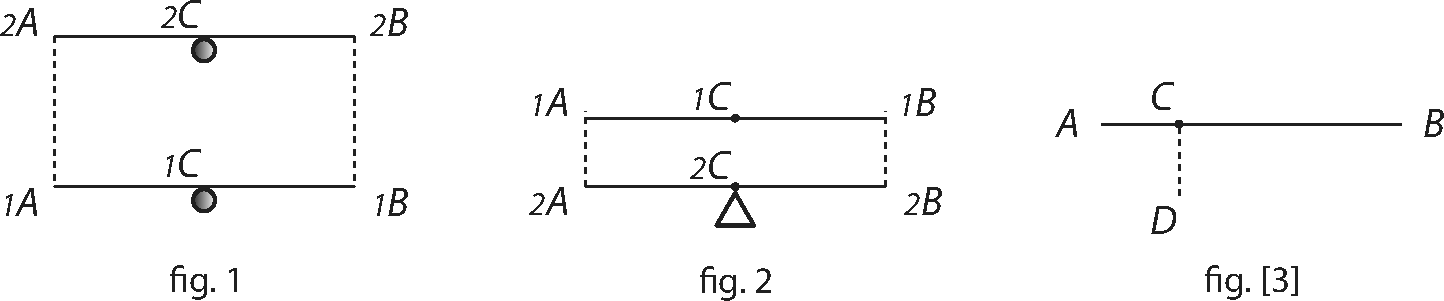
\includegraphics[width=0.96\textwidth]{gesamttex/edit_VIII-4/images/LH_37_05_044_d1-3_044r.pdf}%
\edcaption[-1.25em]%
{%
\edtext{}{\lemma{fig.\,\lbrack3\rbrack}%
\Cfootnote[nonum]{%
In \textit{L} irrtümlich als \textit{fig.\:4} bezeichnet.%
}}%
}%
\end{edfigure}%
\pstart%
\noindent%
\edlabel{LH_37_05_044r_impulsusnonplenus-1}%
Sed cum impulsus%
\indexS{impulsus extra punctum medium}
\edtext{\textit{DC}}{%
\lemma{\textit{DC}}\Bfootnote{%
\textit{erg.\;L}}}
est in puncto \textit{C} extra medium%
\indexS{figura}
\edtext{(fig.\,3),}{%
\lemma{(fig.\,3.)}\Bfootnote{%
\textit{erg.\;L}}}
ibi necesse non est %
ut tota recta%
\indexS{recta recipiens impulsum}
\edtext{\textit{AB} impulsum plene recipiat}{%
\lemma{\textit{AB}}\Bfootnote{%
\textit{(1)}~secundum lineam im
\textit{(2)}~impulsum plene recipiat%
~\textit{L}}}
et quodlibet ejus punctum feratur
nisus gradu \textit{DC}%
\indexS{gradus nisus}
in parallelis ipsi \textit{DC},
nam si
\edtext{punctum \textit{B} vel aliud
in recta \textit{AB} maneret
\lbrack immotum\rbrack\
et}{%
\lemma{punctum}\Bfootnote{%
\textit{B}
\textit{(1)}~manere
\textit{(2)}~vel aliud %
\lbrack...\rbrack\ \textit{AB} maneret
\bars{in motum \textit{ändert Hrsg.}}
et~\textit{L}}}
circa ipsum gyraretur punctum \textit{C} %
ipso nisu recepto,%
\indexS{nisus receptus}
jam impulsui esset satisfactum.%
\edlabel{LH_37_05_044r_impulsusnonplenus-2}
Sed non est rationi consentaneum
ut punctum aliquod in recta \textit{AB} plane quiescat.
Nam si impulsus \textit{C}%
\indexS{impulsus accedens ad punctum medium}
accedat continue versus
\edtext{medium%
\lbrack,\rbrack\
tunc
sive punctum illud quiescens idem maneat
sive continue mutetur%
\lbrack,\rbrack\
utroque modo tunc
continue
acceden\lbrack te\rbrack\
ad medium,%
\indexS{impulsus accedens ad punctum medium}%
}{%
\lemma{medium}\Bfootnote{%
\textit{(1)}~vel
\textit{(2)}~tunc sive punctum illud quiescens
\textit{(a)}~vel
\textit{(b)}~idem
\textit{(aa)}~manebit vel mutabitur
\textit{(bb)}~maneat sive continue mutetur;
\textit{(aaa)}~si enim manet
\textit{(bbb)}~utroque modo tunc continue
\bars{accedendo \textit{ändert Hrsg.}}
ad medium,%
~\textit{L}}}
denique in ipso medio impulsu quoque%
\indexS{impulsus receptus in puncto medio}%
\lbrack,\rbrack\
aliquod maneret punctum quiescens,
quod falsum esse jam
\edtext{constat.
Itaque necesse est
in impulsu Eccentrico%
\indexS{impulsus eccentricus}%
}{%
\lemma{constat.}\Bfootnote{%
\textit{(1)}~Sin punctum quiescens mutetur, tamen aliquod semper
\textit{(a)}~prodibit
\textit{(b)}~erit, etiam impulsus.
\textit{(2)}~Itaque in casu impu
\textit{(3)}~Itaque necesse %
\lbrack...\rbrack\ impulsu Eccentrico%
~\textit{L}}}
motum esse compositum%
\indexS{motus compositus}
ex propulsione%
\indexS{propulsio}
et
\edtext{gyratione.%
\indexS{gyratio in concursu eccentrico}
Et quidem
quo longius recedetur a medio,%
\indexS{impulsus recedens a puncto medio}
hoc magis valebit gyratio,%
\indexS{gyratio in concursu eccentrico}
quo propius ad medium accedetur,%
\indexS{impulsus accedens ad punctum medium}
hoc plus poterit impulsus
donec in medio%
\indexS{impulsus receptus in puncto medio}
omnis gyratio evanescat.%
\indexS{gyratio evanescens}%
}{%
\lemma{gyratione.}\Bfootnote{%
\textit{(1)}~Quod etiam inde \textit{C} vinci potest, quia
\textit{(2)}~Et quidem %
\lbrack...\rbrack\ magis valebit
\textit{(a)}~conatus,
\textit{(b)}~gyratio, quo %
\lbrack...\rbrack\ gyratio evanescat.%
~\textit{L}}}
\pend%
\pstart%
Centrum autem gyrationis%
\indexS{centrum gyrationis}%
\indexS{gyratio in concursu eccentrico}
erit ab ea parte,
quae a puncto impulsus%
\indexS{punctum impulsus}%
\indexS{impulsus eccentricus}
est remotior.
Et accedente puncto impulsus%
\indexS{punctum impulsus}
ad medium,%
\indexS{impulsus accedens ad punctum medium}
etiam centrum gyrationis medio accedet,%
\indexS{centrum gyrationis}
et incidente ipso in medium
\edtext{\lbrack etiam centrum gyrationis in medium\rbrack}{%
\lemma{etiam}\Bfootnote{%
centrum gyrationis in medium
\textit{erg.\;Hrsg.}}}
incidet,
transeunte enim puncto impulsus%
\indexS{punctum impulsus}
in alteram medietatem,
etiam centrum
\edtext{gyrationis%
\indexS{centrum gyrationis}
in priorem medietatem transibit.
Ut in fig.\,4%
\indexS{figura}
si punctum impulsus \textit{C}%
\indexS{punctum impulsus}
sit propius extremo \textit{A},
centrum}{%
\lemma{gyrationis}\Bfootnote{%
in
\textit{(1)}~alteram
\textit{(2)}~priorem medietatem transibit.
\textit{(a)}~Si \textit{C}
\textit{(b)}~Ut
\bars{in fig.\,4 \textit{erg.}}
\textit{(aa)}~si \textit{C} sit propius \textit{A}, cent
\textit{(bb)}~si punctum \lbrack...\rbrack\ \textit{A}, centrum%
~\textit{L}}}
gyrationis \textit{G}%
\indexS{centrum gyrationis}
erit propius extremo \textit{B};
et
\edtext{contra si \textit{C} sit}{%
\lemma{contra}\Bfootnote{%
si
\bars{centrum \textit{gestr.}}
\textit{C} sit%
~\textit{L}}}
propius ipsi \textit{B},
erit \textit{G} propius ipsi \textit{A},
ac proinde si \textit{C} in medio
erit et \textit{G} in medio,
adeoque tunc coincident \textit{G} et \textit{C}.
Sed ipsa gyratio tunc erit infinite parva.%
\indexS{gyratio infinite parva}
\pend%
\pstart%
At inquies,
fateor%
\lbrack,\rbrack\
ostendisti
\edtext{supra}{%
\lemma{supra}\Cfootnote{%
\refpassage{LH_37_05_044r_impulsusnonplenus-1}{LH_37_05_044r_impulsusnonplenus-2}.}}
non sequi
\edtext{necessario nisum}{%
\lemma{necessario}\Bfootnote{%
\textit{(1)}~impulsum
\textit{(2)}~nisum%
~\textit{L}}}
plenum%
\indexS{nisus plenus}
ex impulsu eccentrico;%
\indexS{impulsus eccentricus}
\edtext{attamen nec ostensum est}{%
\lemma{attamen}\Bfootnote{%
\textit{(1)}~nec ostendi
\textit{(2)}~nec ostensum est%
~\textit{L}}}
sequi gyrationem.%
\indexS{gyratio in concursu eccentrico}
Respondeo%
\lbrack:\rbrack\
eo ipso
quod inferri non potest
impulsus plenus,%
\indexS{nisus plenus}
utique nec orietur,
adeoque immiscebit se gyratio,%
\indexS{gyratio immixta}
quae
\edtext{\lbrack ni\-sum\rbrack}{%
\lemma{minus}\Bfootnote{%
\textit{L~ändert Hrsg.}}}
mutat.
Quod ut appareat distinctius %
in omni corpore considerandus est renisus ad motum.%
\indexS{renisus ad motum}
Et perinde est
ac si impulsu facto in \textit{C},%
\indexS{impulsus eccentricus}
reliqua puncta omnia contrarium quendam haberent%
\indexS{nisus contrarius}
\edtext{nisum,
quibus omnibus
posita inflexibilitate%
\indexS{inflexibilitas}
non melius satisfit
\lbrack nisi\rbrack\
per gyrationem.%
\indexS{gyratio immixta}%
}{%
\lemma{nisum,}\Bfootnote{%
\textit{(1)}~ubi sine g
\textit{(2)}~quibus omnibus %
\lbrack...\rbrack\ melius satisfit
\bars{nisi \textit{erg.\;Hrsg.}}
per gyrationem.%
~\textit{L}}}
\pend%
\vspace{1.25em} %
\centerline{%
\includegraphics[width=0.24\textwidth]{%
gesamttex/edit_VIII-4/images/LH_37_05_044_d4_044r.pdf%
}}
\newpage%
\vspace*{0.0em}%
\centerline{\hspace{-55mm}%
\includegraphics[width=0.24\textwidth]{%
gesamttex/edit_VIII-4/images/LH_37_05_044_d5_044r.pdf%
}}%
\vspace{-4.25em} %
\centerline{\hspace{55mm}%
\includegraphics[width=0.24\textwidth]{%
gesamttex/edit_VIII-4/images/LH_37_05_044_d6_044r.pdf%
}}
\vspace{1.0em}
\pstart%
\noindent%
Patet etiam centrum gyrationis \textit{G}%
\indexS{centrum gyrationis}
non esse semper punctum extremum \textit{B};
nam ut ex
\edtext{fig.\,4%
\indexS{figura}
manifestum est,}{%
\lemma{fig.\,4}\Bfootnote{%
\textit{(1)}~patet,
\textit{(2)}~manifestum est,%
~\textit{L}}}
eo propius accedit ad medium,
quo propius ipsum \textit{C} accedit ad medium.
\edlabel{LH_37_05_044_044r_cntrgyr-1}%
Quin imo hinc videtur refutari
\edlabel{LH_37_05_044r_alias_dhe-1}%
quod
\edtext{alias}{%
\lemma{alias}\Cfootnote{%
Wohl N.\;\ref{60142+60297},
\refpassage{60142+60297_centrumgyrationis-1}{60142+60297_centrumgyrationis-2}; siehe auch N.\;\ref{60299}, \refpassage{LH_37_05_043_043v_centrgyr-1}{LH_37_05_043_043v_urzelle-2}.%
}}
mihi rationabile visum est,%
\indexS{rationabile}
centrum gyrationis%
\indexS{centrum gyrationis}
\edtext{(fig.\,5)%
\indexS{figura}
esse centrum gravitatis%
\indexS{centrum gravitatis partis impulsae}
partis non plene impulsae.%
\edlabel{LH_37_05_044r_alias_dhe-2}
Sumatur \textit{AD} portio rectae \textit{AB},
cujus portionis \textit{AD} medium punctum sit \textit{C},%
}{%
\lemma{(fig.\,5)}\Bfootnote{%
\textit{(1)}~esse
\textit{(2)}~ita haberi. Sumatur \textit{CD} aequalis ipsi \textit{CA}
\textit{(3)}~esse centrum \lbrack...\rbrack\ punctum sit \textit{C},%
~\textit{L}}}
in quo fit impulsus,%
\indexS{impulsus eccentricus}
et reliquae partis \textit{DB} medium punctum sit \textit{G}.
Si igitur
\edtext{istud}{%
\lemma{istud}\Bfootnote{%
\textit{erg.\;L}}}
\textit{G} est centrum gyrationis,%
\indexS{centrum gyrationis}
tunc \textit{C} accedente ad medium,
non ideo \textit{G} accedit ad medium,
sed potius accedit ad \textit{B}.
Magis vero rationi consentaneum est%
\indexS{consentaneum rationi}
centrum gyrationis esse \textit{E}%
\indexS{centrum gyrationis}
centrum gravitatis commune%
\indexS{centrum gravitatis commune}
ipsorum \textit{C} et \textit{G},
\edtext{seu centrum gravitatis%
\lbrack,\rbrack%
}{%
\lemma{seu}\Bfootnote{%
centrum gravitatis
\textit{erg.\;L}}}
quoniam \textit{C} incidente in medium
\edtext{tunc \textit{E} etiam}{%
\lemma{tunc}\Bfootnote{%
\textit{(1)}~\textit{G} etiam
\textit{(2)}~\textit{E} etiam%
~\textit{L}}}
incidit in \textit{C}.
Et istud \textit{E} patet
semper esse invariabile seu idem,
ubicunque sit \textit{C}.%
\edlabel{LH_37_05_044_044r_cntrgyr-2}%
\pend%
\pstart%
Omnibus autem expensis
\edtext{talis eventus%
\indexS{eventus}
visus est rationi consentaneus.%
\indexS{consentaneum rationi}
\edlabel{LH_37_05_044r_fig.6-1}%
Incurrat}{%
\lemma{talis}\Bfootnote{%
\textit{(1)}~ratio visa est
\textit{(2)}~eventus visus est rationi consentaneus.
\textit{(a)}~Centrum
\textit{(b)}~Concurrant
\textit{(c)}~Incurrat%
~\textit{L}}}%
\edtext{}{%
\xxref{LH_37_05_044r_fig.6-1}{LH_37_05_044r_fig.6-2}%
\lemma{Incurrat globus \textit{H}}\Cfootnote{%
Vgl. das Diagramm \textit{fig.\,6}.%
}}
globus \textit{H}%
\edlabel{LH_37_05_044r_fig.6-2}
in rectam \textit{AB} quiescentem%
\indexS{globus incurrens in rectam quiescentem}
et incurrat Eccentrice in \textit{C}.%
\indexS{globus incurrens eccentrice}%
\indexS{incursus eccentricus}
\edlabel{LH_37_05_044_044r_navis-1}%
Utique centrum gravitatis eorum%
\indexS{centrum gravitatis commune}
progredietur eodem modo ante et post ictum,%
\indexS{progressus uniformis centri gravitatis}%
\indexS{ictus}
seu salvus erit motus communis%
\indexS{motus communis ut in navi}
quasi in navi ferrentur,%
\indexS{navis}
quae iret motu centri gravitatis.%
\indexS{motus centri gravitatis}%
\edlabel{LH_37_05_044_044r_navis-2}
Et proinde quoad hunc motum communem,%
\indexS{motus communis ut in navi}
ambo ferentur in rectis ipsi \textit{HC} parallelis.
Sed quoad motum proprium%
\indexS{motus proprius}
eadem
\edtext{est vis respectiva}{%
\lemma{est}\Bfootnote{%
\textit{(1)}~motus respectivus
\textit{(2)}~vis respectiva%
~\textit{L}}}
ante et post ictum,%
\indexS{vis respectiva ante ictum}%
\indexS{vis respectiva post ictum}
et \textit{H} quidem reflectitur in linea recta,
at recta \textit{AB} gyratur circa centrum
\edtext{gravitatis \textit{E},%
\indexS{centrum gravitatis commune}
quoniam considerando mobile \textit{AB}
ut reductum in duo puncta \textit{C} et \textit{G},
patet \textit{C} quidem impelli retrorsum
quo tendit \textit{H},
seu directione \textit{HC},
sed \textit{G} non impulsum
\textlangle interim\textrangle\
pergere
ut obstaculo in \textit{C} invento faceret,%
\indexS{obstaculum inventum}
et ita \textit{C} et \textit{G} in diversa nitentibus
gyratio fit%
\indexS{gyratio in concursu eccentrico}
circa centrum gravitatis eorum \textit{E};%
\indexS{centrum gravitatis commune}
ita quidem ut%
}{%
\lemma{gravitatis}\Bfootnote{%
\textit{E}
\textit{(1)}~celeritate
\textit{(2)}~motu reciproce proportionali; ita
\textit{(3)}~, quoniam considerando
\textit{(a)}~corpus
\textit{(b)}~mobile \textit{AB}
\lbrack...\rbrack\ ita quidem
\textit{(aa)}~ut
\textit{(bb)}~ut
\textit{(cc)}~ut%
~\textit{L}}}
motus proprii rectae%
\indexS{recta inflexilis}
et globi%
\indexS{globus incurrens eccentrice}
sint reciproce proportionales%
\indexS{motus proprius}%
\indexS{motus reciproce proportionalis}
ut ante concursum%
\indexS{concursus corporum}%
\lbrack,\rbrack\
tantum quod post ictum%
\indexS{ictus}
ipsius \textit{AB} motus proprius mutatur in gyrationem%
\indexS{motus proprius}%
\indexS{motus mutatus in gyrationem}
manente tamen eadem motus
\lbrack(\protect\vphantom)\rbrack%
\edtext{licet inaequaliter distributi%
\indexS{motus inaequaliter distributus}%
}{%
\lemma{licet}\Bfootnote{%
inaequaliter distributi
\textit{erg.\;L}}}%
\lbrack\protect\vphantom()\rbrack\
quantitate,%
\indexS{quantitas motus eadem}
seu si ex gyratione%
\indexS{gyratio in concursu eccentrico}
fieret motus
\edtext{rectus aequidistributus parallelus,%
\indexS{motus aequidistributus}%
\indexS{motus rectus}
centrum gravitatis \textit{E}%
\indexS{centrum gravitatis commune}
adeoque et tota \textit{AB} ferretur%
}{%
\lemma{rectus}\Bfootnote{%
\textit{(1)}~centrum gravitatis \textit{E} feretu
\textit{(2)}~aequidistributus parallelus, \lbrack...\rbrack\ \textit{AB} ferretur%
~\textit{L}}}
celeritate%
\indexS{celeritas reciproca}
\edtext{reciproca ad eam
qua}{%
\lemma{reciproca}\Bfootnote{%
\textit{(1)}~ad eam qu
\textit{(2)}~\bars{quantitatis \textit{streicht Hrsg.}}
\textit{(3)}~ad eam qua%
~\textit{L}}}
\textit{H} globus,%
\indexS{globus incurrens eccentrice}
itaque centra gravitatis%
\indexS{centrum gravitatis partis percussae}
\edtext{\textit{C}}{%
\lemma{\textit{C}}\Bfootnote{%
\textit{erg.\;L}}}
partis plene percussae \textit{AD} %
et \textit{G} partis non plene percussae \textit{DB} %
\indexS{centrum gravitatis partis percussae}
\edtext{gyrantur circa centrum totius \textit{E},%
\indexS{centrum gravitatis commune}
celeritatibus etiam}{%
\lemma{gyrantur}\Bfootnote{%
\textit{(1)}~etiam
\textit{(2)}~circa centrum %
\lbrack...\rbrack\ celeritatibus etiam%
~\textit{L}}}
reciproce proportionalibus%
\indexS{celeritas reciproce proportionalis}%
\lbrack;\rbrack\
et ducta quavis parte in celeritatem sui centri,%
\indexS{celeritas centri gravitatis}
prodit quantitas motus%
\indexS{quantitas motus eadem}
ex summa %
aequalis ei quam habet \textit{H}.%
\pend%
\pstart%
Sed succurrit tamen dubitatio%
\indexS{dubitatio}
quoad celeritatem reciproce proportionalem%
\indexS{celeritas reciproce proportionalis}
seu eandem quantitatem motus ipsius \textit{AB}%
\indexS{quantitas motus eadem}
et ipsius~\textit{H},
nam ita verum est quidem in motu aequidistributo%
\indexS{motus aequidistributus}
eandem prodire potentiam%
\indexS{potentia eadem}
\edtext{ex vi directionis%
\indexS{vis directionis}
et vi respectiva seu percussionis;%
\indexS{vis respectiva}%
\indexS{vis percussionis}%
}{%
\lemma{ex}\Bfootnote{%
\textit{(1)}~summa motus recti
\textit{(2)}~vi directionis \lbrack...\rbrack\ seu percussionis;%
~\textit{L}}}
sed hic videndum
an etiam absolutos motus considerando,%
\indexS{motus absolutus}
eadem hinc prodeat potentia absoluta%
\indexS{potentia absoluta}%
\indexS{potentia eadem}
in concursu Eccentrico%
\indexS{concursus eccentricus}%
\lbrack;\rbrack\
quod magnum foret indicium veritatis.%
\indexS{indicium veritatis}%
\indexS{veritas}
\lbrack%
\href{\Scan{LH_37_05_044v}}%
{44\,v\textsuperscript{o}\rbrack}%
\rbrack%
\pend%
\pstart%
Hinc etiam illud sequitur perpulchrum%
\lbrack:\rbrack\
omnes Eccentricos impulsus%
\indexS{impulsus eccentricus}
facere gyrationem%
\indexS{gyratio circa centrum gravitatis}
circa idem centrum.%
\indexS{centrum gyrationis}
Hinc si sint
\edtext{simul}{%
\lemma{simul}\Bfootnote{%
\textit{erg.\;L}}}
ad easdem partes augere gyrum,%
\indexS{gyrus}
sin
\edtext{minus e\lbrack u\rbrack m minuere.
Id quomodo fiat determinandum,
ut appareat quatenus unde augeatur repercussio,%
\indexS{repercussio}%
}{%
\lemma{minus}\Bfootnote{%
\bars{eam \textit{ändert Hrsg.}}
minuere
\textit{(1)}~, aucta repercussione
\textit{(2)}~. Id quomodo %
\lbrack...\rbrack\ augeatur repercussio,%
~\textit{L}}}
et quid omnino prodeat.%
\pend%
\selectlanguage{latin}%
\frenchspacing%
\normalsize%
